\documentclass[12pt]{article}

% Codificación y lenguaje
\usepackage[utf8]{inputenc}
\usepackage[T1]{fontenc}
\usepackage[spanish]{babel}
\usepackage{tikz}
\usetikzlibrary{positioning, arrows.meta}
\usepackage{graphicx} 

% Márgenes
\usepackage[a4paper, left=2.5cm, right=2.5cm, top=2cm, bottom=2cm]{geometry}

% Gráficos, flotantes y código
\usepackage{graphicx}
\usepackage{float}
\usepackage{listings}
\usepackage{xcolor}
\usepackage{tikz}
\usepackage{url}
\usepackage{hyperref}

% Encabezados y pies de página
\usepackage{fancyhdr}
\pagestyle{fancy}
\fancyhf{}
\lhead{TP Nº1 - Muestreo de señales}
\rhead{UNC-Procesamiento digital de señales}
\cfoot{\thepage}

% Estilo para código Matlab
\definecolor{codegreen}{rgb}{0,0.6,0}
\definecolor{codegray}{rgb}{0.5,0.5,0.5}
\definecolor{codepurple}{rgb}{0.58,0,0.82}
\definecolor{backcolour}{rgb}{0.95,0.95,0.92}

\lstdefinestyle{mystyle}{
	language=C,
	backgroundcolor=\color{white},
	basicstyle=\scriptsize\ttfamily,           % Tamaño de fuente reducido con tipografía monoespaciada
	keywordstyle=\color[HTML]{0072BD}\bfseries,
	commentstyle=\color[HTML]{008000}\itshape,
	stringstyle=\color[HTML]{A2142F},
	numberstyle=\tiny\color{gray},             % Números de línea discretos
	numbers=left,
	numbersep=6pt,                             % Separación más generosa para claridad
	frame=single,
	rulecolor=\color{black!50},
	breaklines=true,                           % Cortar líneas largas automáticamente
	breakatwhitespace=false,                   % Cortar incluso sin espacios
	breakautoindent=true,                      % Mantener indentación visual
	tabsize=2,
	showspaces=false,
	showstringspaces=false,
	xleftmargin=1.5em,                         % Margen izquierdo para números
	xrightmargin=0.5em,
	aboveskip=1em,                             % Espacio antes del bloque de código
	belowskip=1em,                             % Espacio después del bloque de código
}


% Título y autores
\title{
	
\includegraphics[width=0.45\textwidth]{unc.png} \\[2cm] % Logo
	\textbf{Trabajo Práctico Nº1: Muestreo de señales}
}

\author{
	Profesores: \\ Parlanti Gustavo Fernand (Presidente) \\ Molina German Alcides (Vocal)\\ Rossi Robreto Raul (Vocal)
	\\ \\
	Alumnos:\\ Campos \\ Testa \\ Verstraete 
}

\date{Mayo de 2025} % Fecha del trabajo

\begin{document}
	
	\maketitle
	
	\begin{abstract}
	 Realizar un programa aplicativo que sea capaz de digitalizar una señal a través del modulo del ADC disponible en la placa de desarrollo a distintas velocidades de muestreo, las  requeridas son 8K/S, 16K/S 22K/S, 44K/S y 48K/S. Los cambios de las velocidades de muestreo serán realizados con una de las teclas de la placa de evaluación, en forma de un buffer circular. Cada velocidad de muestreo se indicará a través de un color RGB del LED. Con otra tecla de la placa se habilitara la adquisición o se parara la misma (Run/Stop). Los valores adquiridos serán almacenados en memoria en un buffer circular de 512 muestras del tipo q15 (fraccional 15bits) y a su vez serán enviados a través del DAC (de 12bits).
	\end{abstract}\newpage
	
	\tableofcontents \newpage
	
	\section{Introducción}
	En los sistemas embebidos modernos, la digitalización de señales analógicas en tiempo real representa una funcionalidad crítica en aplicaciones como adquisición de datos, procesamiento digital de audio, control industrial y sistemas de comunicación. Este trabajo práctico tiene como objetivo principal el desarrollo de un sistema aplicativo que implemente un flujo completo de adquisición, procesamiento y reproducción de señales analógicas en una placa de desarrollo basada en un microcontrolador STM32F446RE.
	
	El sistema propuesto permite capturar una señal analógica utilizando el módulo ADC (Convertidor Analógico-Digital) del microcontrolador, convertir los valores a formato Q15 (15 bits fraccional en punto fijo), y almacenarlos en un buffer circular de 512 muestras. Posteriormente, estas  son reproducidas en tiempo real mediante el módulo DAC (Convertidor Digital-Analógico) integrado en la misma placa. Todo el proceso se realiza en tiempo real y bajo distintas velocidades de muestreo, seleccionables dinámicamente mediante una interrupción de GPIO.
	
	\subsection{Objetivos del proyecto}
	
	\begin{itemize}
		 \item Implementar la digitalización de señales en tiempo real utilizando el ADC de la placa STM32F446RE.
		 
		 \item Diseñar e integrar un buffer circular para almacenar muestras en formato Q15, asegurando un flujo continuo de datos sin pérdidas.
		 
		 \item Configurar y utilizar el DAC para la reproducción de la señal adquirida.
		 
		 \item Permitir el cambio dinámico de la frecuencia de muestreo (8 kHz, 16 kHz, 22 kHz, 44 kHz y 48 kHz) mediante una tecla de usuario, utilizando una estructura de tipo circular.
		 
		 \item Utilizar un LED RGB como indicador visual de la frecuencia de muestreo seleccionada.
		 
		 \item Implementar una segunda tecla que permita habilitar o detener el proceso de adquisición y reproducción (modo Run/Stop).
		 
		 \item Optimizar el sistema para que funcione de manera eficiente utilizando DMA (Acceso Directo a Memoria) y temporizadores (TIM) del microcontrolador.
	\end{itemize}
	
	\subsection{Aspectos relevantes a tener en cuenta}
	Para lograr una digitalización y reproducción de señales eficiente y en tiempo real, se implementaron varias técnicas clave orientadas a minimizar la latencia, reducir la carga del procesador y mejorar la capacidad de respuesta del sistema. A continuación se describen los principales enfoques adoptados:
	
	\subsubsection{Uso de DMA (Direct Memory Access)}
	El DMA permite que los datos capturados por el ADC y enviados al DAC sean transferidos directamente entre periféricos y memoria sin intervención del CPU. Esta técnica es esencial para evitar interrupciones por cada muestra y reducir drásticamente la latencia en la adquisición y reproducción de señales, permitiendo que el procesador se enfoque exclusivamente en tareas de control o procesamiento si es necesario.\newpage
	
	\begin{itemize}
		\item En el sistema implementado, tanto el ADC como el DAC trabajan en modo DMA.
		
		\item Las transferencias se configuran en modo circular para que una vez completado el buffer, el periférico vuelva automáticamente al inicio.
	\end{itemize}
	
	\subsubsection{Técnica de Doble Buffering (Ping-Pong Buffer)}
	Para asegurar una reproducción continua y evitar glitches o corrupción de datos en la señal de salida, se implementó una técnica de doble buffering. En este esquema, el buffer de 512 muestras se divide en dos mitades:
	
	\begin{itemize}
		\item Mientras el ADC llena una mitad del buffer,la otra mitad procesa los datos obtenidos, en este caso los transforma a Q15 y los adapta para sacar la señal por el DAC
		
		\item Al completarse una transferencia, se realiza el "ping-pong" de roles entre mitades.
	\end{itemize}
	
	Esta técnica permite una transición fluida entre adquisición y reproducción, eliminando tiempos muertos y mejorando la latencia total del sistema.
	
	\subsubsection{Medición del Tiempo de Procesamiento con el Módulo DWT}
	Para evaluar el rendimiento del sistema y optimizar su eficiencia, se utilizó el módulo DWT (Data Watchpoint and Trace Unit) disponible en el microcontrolador STM32F446RE. Este módulo permite acceder al registro CYCCNT, que cuenta ciclos de CPU con alta resolución.
	
	\begin{itemize}
		\item Se utilizó para medir el tiempo exacto de procesamiento por bloque de datos (por ejemplo, el tiempo entre interrupciones DMA half-complete y complete).
		
		\item Permite realizar profiling en tiempo real, identificando cuellos de botella en el flujo de datos y verificando que el sistema cumple con las restricciones temporales para cada frecuencia de muestreo.
		
		\item Esta métrica es fundamental para garantizar el correcto funcionamiento incluso a altas tasas de muestreo como 48kHz.
	\end{itemize}
	
	\section{Marco teórico}
	El procesamiento digital de señales (DSP) en sistemas embebidos se basa en principios matemáticos y físicos que permiten representar y manipular señales analógicas en forma digital. Esta sección revisa los conceptos esenciales relacionados al muestreo, la reconstrucción de señales, y su representación numérica, todos fundamentales para el desarrollo de aplicaciones de adquisición y reproducción de señales en tiempo real.
	
	\subsection{Señales continuas y discretas}
	Una señal analógica es una función continua en el tiempo que puede tomar un conjunto infinito de valores. En contraste, una señal discreta en el tiempo se define sólo en instantes específicos (secuenciales), y una señal digital es aquella que además tiene valores cuantificados (por ejemplo, números enteros o punto fijo).
	Para poder procesar una señal analógica en un sistema digital es necesario muestrearla y cuantizarla:
	
	\begin{itemize}
		\item Muestreo: tomar valores de la señal a intervalos de tiempo regulares $T_{s} = \frac{1}{f_{s}}$
		\item Cuantización: representar cada muestra con un número finito de bits 
	\end{itemize}
	
	\subsection{Teorema de Nyquist-Shannon}
	El Teorema de Muestreo de Nyquist-Shannon establece que una señal analógica de ancho de banda limitado $f_{max}$ puede ser reconstruida perfectamente a partir de sus muestras si se cumple:
	
	\begin{equation}
		f_{s} \geq 2 f_{max}
	\end{equation}
	
	Si se muestrea por debajo de este umbral, ocurre aliasing, es decir, componentes de alta frecuencia se pliegan en el espectro y aparecen como señales falsas en bajas frecuencias.
	
	\subsection{Reconstrucción de señales}
	La reconstrucción de una señal analógica a partir de sus muestras digitales implica generar una versión continua en el tiempo que se asemeje lo más posible a la señal original. En teoría, esto se logra mediante interpolación ideal con funciones sinc, lo cual no es factible en sistemas reales debido a su complejidad infinita. En la práctica, se utilizan filtros pasa bajos analógicos a la salida del DAC para suavizar la señal escalonada producida por la conversión digital-analógica. La calidad de esta reconstrucción depende de factores como la frecuencia de muestreo utilizada, la resolución de cuantización, y la respuesta del filtro reconstructivo. En sistemas embebidos, esta etapa es crítica en aplicaciones de audio o instrumentación, donde se requiere fidelidad y baja distorsión.
	
	\subsection{Procesamiento Digital en Sistemas Embebidos}
	El procesamiento digital de señales (DSP) en sistemas embebidos implica trabajar con muestras digitalizadas para realizar operaciones como filtrado, transformación, detección o generación de señales. Dado que los microcontroladores suelen tener recursos limitados (memoria, velocidad, consumo), se emplean técnicas optimizadas como el uso de formato Q15, que representa números fraccionarios en punto fijo de 16 bits, permitiendo una aritmética rápida sin necesidad de FPU. Además, se emplean periféricos como DMA para transferencias de datos sin intervención del CPU, y temporizadores para garantizar una temporización precisa en la adquisición y reproducción. Este enfoque permite realizar procesamiento en tiempo real en aplicaciones como audio digital, monitoreo de sensores o control en lazo cerrado.
	Una vez digitalizada, la señal puede ser procesada con algoritmos de DSP, como:
	
	\begin{itemize}
		\item Filtros digitales (FIR, IIR)
		
		\item Transformadas rápidas (FFT)
		
		\item Compresión o codificación
	\end{itemize}\newpage
	
	\subsection{CMSIS-DSP}
	
	La biblioteca \textbf{CMSIS-DSP} (Cortex Microcontroller Software Interface Standard - Digital Signal Processing) es una colección de funciones optimizadas desarrolladas por ARM para facilitar el procesamiento de señales digitales en microcontroladores basados en núcleos Cortex-M. Esta biblioteca forma parte del ecosistema CMSIS y proporciona una API estandarizada que incluye operaciones matemáticas básicas, filtros FIR e IIR, transformadas rápidas de Fourier (FFT), convoluciones, correlaciones, estadísticas y operaciones vectoriales, todas implementadas en código eficiente y adaptado al hardware.
	
	Una de las principales ventajas de CMSIS-DSP es que ofrece rutinas en formato \texttt{fixed-point} (\texttt{Q15} y \texttt{Q31}) y \texttt{floating-point}, lo cual permite su uso tanto en microcontroladores sin unidad de punto flotante como en aquellos que sí la poseen (por ejemplo, los basados en Cortex-M4 y Cortex-M7 con FPU).
	
	Estas funciones están altamente optimizadas en ensamblador para los núcleos ARM, aprovechando instrucciones SIMD (Single Instruction, Multiple Data) y otras características de hardware, logrando un alto rendimiento con un bajo consumo de recursos.
	
	\section{Placa de Desarrollo y Herramientas Utilizadas}
	El proyecto fue desarrollado sobre la placa STM32 Nucleo-F446RE, basada en el microcontrolador STM32F446RE, perteneciente a la familia STM32F4 de STMicroelectronics. Esta plataforma integra una arquitectura avanzada ARM Cortex-M4, periféricos orientados a procesamiento de señales, y herramientas de desarrollo que permiten implementar sistemas en tiempo real de forma eficiente.
	
	\begin{figure}[h!]
		\centering
		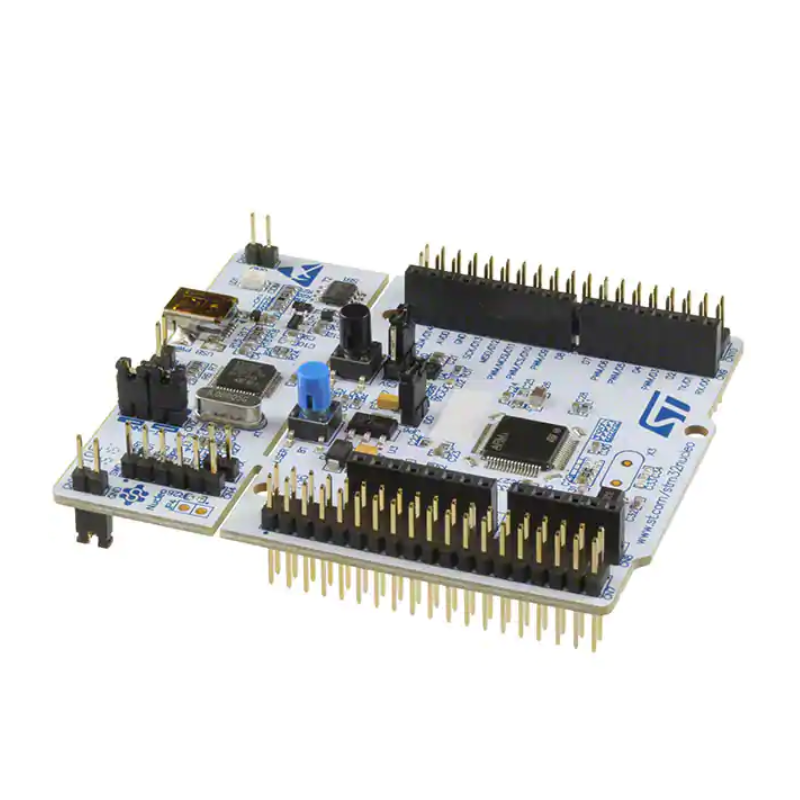
\includegraphics[width=0.7\linewidth]{placa}
		\caption[Placa de desarrollo]{Placa de desarrollo}
		\label{fig:placa}
	\end{figure}
	
	\subsection{Microcontrolador STM32F446RE}
	El STM32F446RE es un microcontrolador de 32 bits basado en el núcleo ARM Cortex-M4, optimizado para procesamiento digital con soporte de instrucciones DSP y unidad de punto flotante opcional (FPU simple precisión). Sus principales características relevantes al proyecto son:
	
	\begin{itemize}
		\item Frecuencia de operación: hasta 180MHz
		
		\item Memoria Flash: 512KB
		
		\item RAM: 128KB
		
		\item Tensión de operación: 1.8V a 3.6V
		
		\item Paquete: LQFP64 (compatible con la Nucleo-F446RE)
	\end{itemize}
	
	\subsection{Núcleo ARM Cortex-M4}
	El núcleo ARM Cortex-M4 es el corazón del microcontrolador STM32F446RE y está especialmente diseñado para aplicaciones que requieren una combinación de procesamiento eficiente, bajo consumo y capacidad de ejecución de algoritmos DSP (procesamiento digital de señales) en tiempo real. Se trata de una arquitectura de 32 bits basada en el conjunto de instrucciones Thumb-2, que combina instrucciones de 16 y 32 bits para mejorar la eficiencia del código y reducir el uso de memoria, una característica especialmente valiosa en sistemas embebidos con recursos limitados.
	
	Una de las principales ventajas del Cortex-M4 respecto de sus predecesores es su capacidad nativa de ejecutar instrucciones DSP, como multiplicación acumulada (MAC, Multiply-and-Accumulate), operaciones SIMD (Single Instruction Multiple Data), y saturación aritmética, lo cual lo convierte en una excelente opción para aplicaciones de filtrado digital, transformadas rápidas (FFT) y otras tareas típicas de procesamiento de señales. Estas instrucciones están directamente soportadas por el compilador y son aceleradas por hardware, lo que reduce el número de ciclos por operación y mejora considerablemente el rendimiento en tiempo real.
	
	El Cortex-M4 también incluye un sistema de interrupciones NVIC altamente eficiente, que permite la respuesta rápida a eventos críticos como interrupciones del ADC, botones o DMA, lo cual es fundamental en aplicaciones que requieren tiempos deterministas. Además, incorpora el módulo DWT (Data Watchpoint and Trace), que ofrece herramientas de diagnóstico avanzadas como el contador de ciclos de CPU (CYCCNT), ideal para realizar mediciones de tiempo precisas, evaluación de latencia y profiling de código sin necesidad de hardware externo.
	
	Aunque algunos modelos de Cortex-M4 incluyen una unidad de punto flotante (FPU) de precisión simple, en este proyecto se optó por trabajar con formato Q15 (punto fijo) para maximizar la eficiencia y mantener la compatibilidad con la biblioteca CMSIS-DSP, que explota al máximo las capacidades nativas del núcleo para operar en enteros fraccionales.
	
	\subsection{Periféricos clave utilizados}
	\subsubsection{ADC (Analog-to-Digital Converter)}
	El STM32F446RE cuenta con 3 ADCs independientes (ADC1, ADC2 y ADC3), cada uno de 12 bits de resolución y con capacidad de hasta 2.4 MSPS (mega muestras por segundo) en modo intercalado. Para este proyecto se utiliza el ADC1 en modo regular y con DMA activado. Sus características técnicas relevantes incluyen:
	
	\begin{itemize}
		\item Resolución seleccionable: 6, 8, 10 o 12 bits (se usa 12 bits para mayor precisión).
		
		\item Tasa de muestreo máxima (single conversion): hasta 2.4 MSPS.
		
		\item Rango de entrada: 0V a VREF (típicamente 3.3V).
		
		\item Tiempo de muestreo configurable: desde 3 hasta 480 ciclos de ADC.
		
		\item Trigger externo: el inicio de la conversión puede ser disparado por un temporizador, lo cual permite muestrear a frecuencias precisas.
		
		\item Modo DMA: transferencia automática de los resultados a un buffer en memoria (sin intervención del CPU).
		
		\item Modo continuo + DMA circular: permite muestreo ininterrumpido con mínimo overhead.
	\end{itemize}
	
	\subsubsection{DAC (Digital-to-Analog Converter)}
	El STM32F446RE incluye 2 canales DAC (DAC1 y DAC2), ambos de 12 bits, con capacidad de salida en modo bufferizado (con baja impedancia) o sin buffer (alta velocidad). Se utiliza DAC1 en este proyecto para convertir las muestras digitales de salida nuevamente en una señal analógica. Características clave:
	
	\begin{itemize}
		\item Resolución de conversión: 12, 10 u 8 bits.
		
		\item Velocidad típica: hasta 1 MSPS (modo sin buffer).
		
		\item Modo bufferizado: reduce el ruido, ideal para salidas de audio.
		
		\item Trigger externo: puede sincronizarse con un temporizador (por ejemplo TIM6/TRGO).
		
		\item Soporte DMA: se permite la alimentación directa de datos desde memoria al DAC sin CPU.
		
		\item Salidas disponibles: a través de pines analógicos dedicados (por ejemplo, PA4 para DAC1).
	\end{itemize}
	
	\subsubsection{DMA (Direct Memory Access)}
	El controlador DMA2 es utilizado para las transferencias entre ADC/DAC y RAM. El STM32F446RE cuenta con dos controladores DMA (DMA1 y DMA2), con un total de 16 canales (streams) y soporte para múltiples periféricos. Características específicas:
	
	\begin{itemize}
		\item Transferencia en background, sin intervención del CPU.
		
		\item Modo circular: ideal para buffers cíclicos o doble buffering.
		
		\item Prioridad programable por canal.
		
		\item Transferencia por palabras (16 bits en Q15).
		
		\item Eventos por mitad de buffer y buffer completo: permite usar doble buffer sincronizado.
	\end{itemize}
	
	\subsubsection{TIM (Timers)}
	El STM32F446RE cuenta con 14 temporizadores (4 avanzados, 2 básicos, 8 generales), todos con configuraciones de prescaler, auto-reload y posibilidad de generar eventos de actualización. Se utilizan para generar señales periódicas que actúan como trigger de muestreo. Características clave:
	\begin{itemize}
		\item TIM2-TIM5: de 32 bits, con amplio rango de conteo (útiles para precisión en frecuencias bajas).
		
		\item Configuración de frecuencia: vía Prescaler y ARR (Auto-Reload Register).
		
		\item Trigger de ADC/DAC: mediante señal TRGO (Trigger Output).
		
		\item Modo master-slave: permite sincronización entre periféricos.
	\end{itemize}
	
	\subsubsection{GPIO – General Purpose Input/Output}
	Los pines GPIO permiten la interacción con el usuario mediante botones (teclas) y LEDs. Se utilizan:
	
	\begin{itemize}
		\item Velocidad de salida seleccionable: Low, Medium, Fast, High.
		
		\item Pull-up/Pull-down configurables.
		
		\item Interrupciones por flanco ascendente, descendente o ambos.
	\end{itemize}
	
		\subsubsection{Herramientas de desarrollo}
	Para la implementación del proyecto se utilizaron las siguientes herramientas:
	
	\begin{itemize}
		\item STM32CubeIDE: entorno de desarrollo oficial de STMicroelectronics, basado en Eclipse, que permite configurar periféricos gráficamente, generar código y compilar con GCC.
		
		\item STM32CubeMX: herramienta para la configuración inicial de pines, relojes, periféricos y generación de código base.
		
		\item CMSIS y CMSIS-DSP: bibliotecas proporcionadas por ARM para facilitar el uso de instrucciones de bajo nivel y rutinas DSP optimizadas en punto fijo.
		
		\item GDB y ST-Link: utilizados para depuración, profiling y medición de tiempos mediante DWT->CYCCNT.
	\end{itemize}\newpage
	
	\begin{figure}[h!]
		\centering
		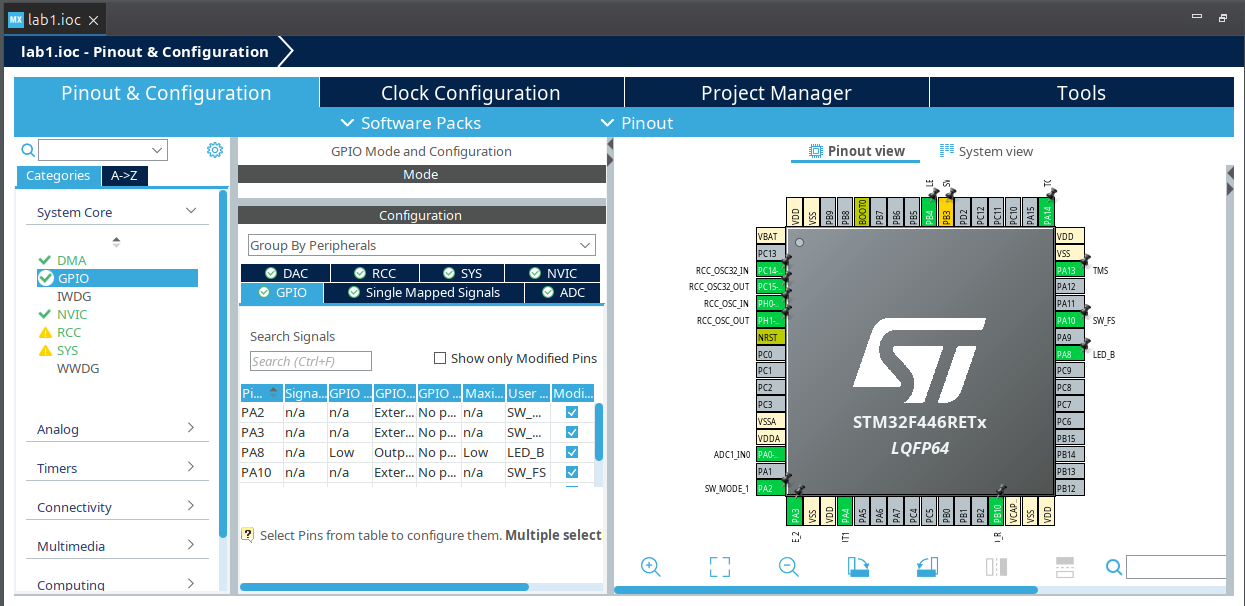
\includegraphics[width=1\linewidth]{IDE}
		\caption[Entorno de desarrollo STM32CUBE IDE]{Entorno de desarrollo STM32CUBE IDE}
		\label{fig:ide}
	\end{figure}
	
	
	
	\section{Diseño del sistema}
	
	\subsection{Descripción detallada del funcionamiento}
	El flujo de datos comienza con la conversión analógica-digital realizada por el ADC1, configurado en modo de escaneo continuo y disparado por el temporizador TIM2. El resultado de estas conversiones es almacenado directamente en el buffer \texttt{adc\_buffer} mediante DMA en modo circular, lo cual permite una operación ininterrumpida sin intervención del procesador. El buffer es de tipo doble (double-buffered), con interrupciones generadas al completar la mitad y el total del buffer, utilizando los callbacks \texttt{HAL\_ADC\_ConvHalfCpltCallback} y \texttt{HAL\_ADC\_ConvCpltCallback}, respectivamente.
	
	Cada vez que se activa uno de estos callbacks, se llama a la función \texttt{process\_buffer\_half}, la cual toma la mitad correspondiente del buffer de entrada, realiza la conversión a formato Q15 (\texttt{q15\_t}) y, opcionalmente, podría aplicar un procesamiento digital (aunque en este código no se incluye ningún filtro). Posteriormente, los datos en Q15 son convertidos al formato requerido por el DAC de 12 bits mediante la función \texttt{convert\_q15\_to\_dac\_buffer}, la cual realiza un escalado proporcional y recorte para mantener los valores en el rango [0, 4095]. El resultado se almacena en \texttt{dac\_buffer} y se reproduce a través del canal 1 del DAC, también utilizando DMA.
	
	Un aspecto destacable del sistema es el uso del contador de ciclos del DWT (\texttt{Data Watchpoint and Trace}) para medir el tiempo exacto de procesamiento de cada mitad del buffer. Este contador se activa en el \texttt{main} y se lee al principio y final de cada ejecución de \texttt{process\_buffer\_half}, almacenando la diferencia en la variable global \texttt{time}. Esta métrica resulta útil para analizar el rendimiento del sistema o para evaluar el impacto del procesamiento DSP si se agregan etapas de filtrado más adelante.
	
	El sistema también incluye un mecanismo de selección de frecuencia de muestreo a través de una interrupción externa generada por un pulsador conectado al pin \texttt{SW\_FS}. Cada vez que se detecta una pulsación, se incrementa el valor del modo de muestreo \texttt{fs\_mode}, recorriendo un ciclo de seis estados. En cada modo, se actualiza el valor de auto-recarga del temporizador TIM2 (\texttt{ARR}) para modificar la frecuencia de disparo del ADC, alcanzando frecuencias de muestreo aproximadas de 8 kHz, 16 kHz, 24 kHz, 40 kHz y 48 kHz. El sexto modo detiene por completo el muestreo, apagando el temporizador y apagando todos los LEDs indicadores.
	
	Los LEDs conectados a los pines \texttt{LED\_B}, \texttt{LED\_R} y \texttt{LED\_G} actúan como indicadores visuales del modo actual de frecuencia de muestreo. Esto permite al usuario reconocer rápidamente el estado del sistema sin requerir una interfaz adicional.
	
	La función \texttt{main} inicializa los periféricos esenciales mediante llamadas generadas por CubeMX: ADC, DAC, DMA, GPIO y el temporizador TIM2. Luego activa el sistema de temporización, inicia la conversión del ADC en modo DMA, así como la salida del DAC también por DMA, y deja el bucle principal completamente vacío. Todo el flujo de datos y procesamiento se lleva a cabo de manera asíncrona mediante interrupciones y DMA, garantizando una alta eficiencia y baja latencia.
	
	Este enfoque modular, escalable y eficiente lo convierte en una base robusta para sistemas de procesamiento de señal embebido, como filtros en tiempo real, analizadores de espectro o codificadores de audio, con la posibilidad de extender fácilmente su funcionalidad agregando etapas DSP en el dominio Q15 aprovechando la biblioteca CMSIS-DSP.
	
	\subsection{Diagrama de bloques del programa aplicativo}
	El siguiente diagrama de bloques resume el flujo funcional del sistema de adquisición y reproducción de señales en tiempo real.
	
	\begin{figure}[h]
		\centering
		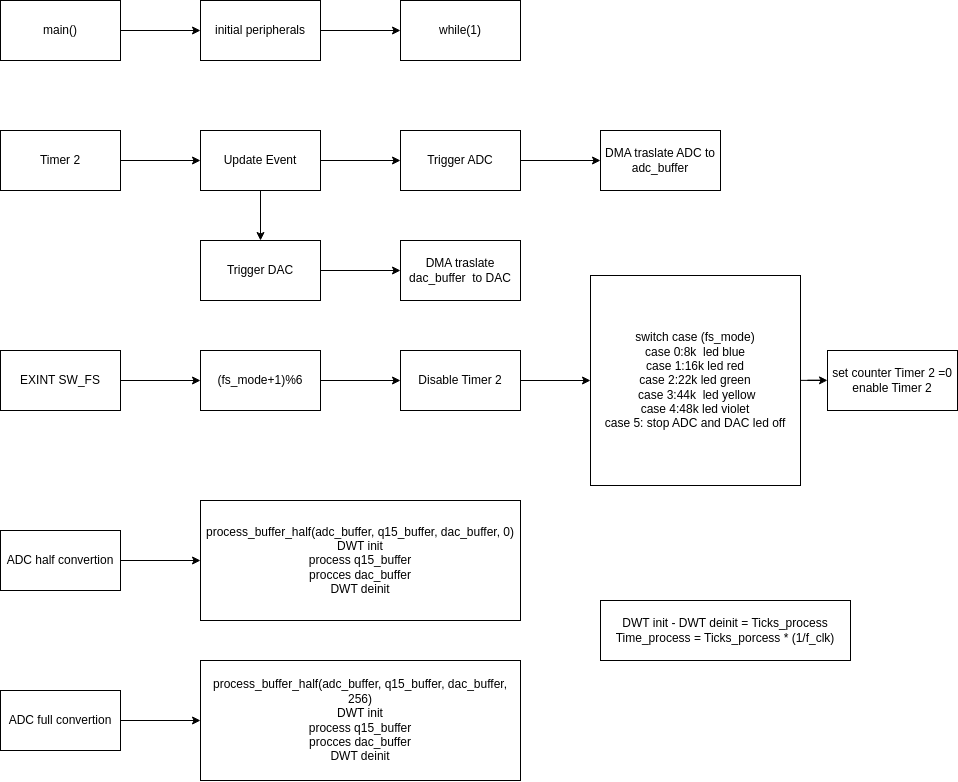
\includegraphics[width=1\linewidth]{lab1_dps.drawio}
		\caption[Diagrama de flujo TOP LEVEL]{Diagrama de flujo TOP LEVEL}
		\label{fig:lab1dps}
	\end{figure}\newpage
	
	\section{Programa principal}
	
	\subsection{Implementación del main.c}
    \begin{lstlisting}[style=mystyle]
		/**
		**********************************************************
		* @file           : main.c
		* @brief          : Real-Time ADC Sampling and Playback via DAC using DMA
		*
		* This program performs real-time signal acquisition and playback on the STM32F446RE
		* microcontroller. It continuously samples an analog input signal using the ADC,
		* converts the samples to Q15 fixed-point format, and reproduces them via the DAC.
		* The entire process is handled using DMA and operates in a double-buffered fashion
		* to ensure minimal CPU usage. The system includes a performance profiling mechanism
		* based on the DWT cycle counter.
		*
		* Key Features:
		* - 12-bit ADC sampling with DMA in circular mode
		* - Q15 fixed-point format conversion
		* - 12-bit DAC output via DMA
		* - Processing time measurement using DWT->CYCCNT
		* - Configurable sampling frequency via TIM2
		*
		* Author          : Campos Mariano
		* Date            : 25/06/2025
		***********************************************************
		*/
		
		/* USER CODE END Header */
		/* Includes ------------------------------------------------------------------*/
		#include "main.h"
		#include "adc.h"
		#include "dac.h"
		#include "dma.h"
		#include "tim.h"
		#include "gpio.h"
		
		/* Private includes ----------------------------------------------------------*/
		/* USER CODE BEGIN Includes */
		#include "arm_math.h" // CMSIS-DSP library for fixed-point processing
		/* USER CODE END Includes */
		
		/* Private typedef -----------------------------------------------------------*/
		/* USER CODE BEGIN PTD */
		
		/* USER CODE END PTD */
		
		/* Private define ------------------------------------------------------------*/
		/* USER CODE BEGIN PD */
		#define BUFFER_SIZE 512     // Size of ADC/DAC/Q15 buffers
		#define FS_8K   11249       // Auto-reload value for TIM2 to achieve ~8kHz sampling with 90 MHz clock
		/* USER CODE END PD */
		
		/* Private variables ---------------------------------------------------------*/
		
		/* USER CODE BEGIN PV */
		extern TIM_HandleTypeDef htim2;      // Timer used for triggering ADC/DAC
		extern ADC_HandleTypeDef hadc1;      // ADC handle
		extern DAC_HandleTypeDef hdac;       // DAC handle
		
		uint16_t adc_buffer[BUFFER_SIZE];    // Raw ADC samples
		uint16_t dac_buffer[BUFFER_SIZE];    // Output buffer for DAC
		q15_t q15_buffer[BUFFER_SIZE];       // Intermediate Q15 format buffer
		uint8_t fs_mode = 0;                 // Sampling frequency mode selector
		uint32_t time = 0;                   // Variable to store CPU cycles for processing time profiling
		/* USER CODE END PV */
		
		/* Private user code ---------------------------------------------------------*/
		/* USER CODE BEGIN 0 */
		
		/**
		* @brief Converts a Q15 array to a 12-bit DAC buffer
		* @param in: Input Q15 data array
		* @param out: Output DAC buffer
		* @param len: Number of elements to convert
		*/
		void convert_q15_to_dac_buffer(q15_t *in, uint16_t *out, uint16_t len) {
			for (uint16_t i = 0; i < len; i++) {
				int32_t val = ((int32_t) in[i] * 4095) / 32767;
				if (val < 0)
				val = 0;
				else if (val > 4095)
				val = 4095;
				out[i] = (uint16_t) (val);
			}
		}
		
		/**
		* @brief Processes half of the ADC buffer: converts to Q15, applies processing, and prepares DAC output
		* @param adc_in: Input ADC buffer
		* @param q15_out: Intermediate Q15 buffer
		* @param dac_out: Output DAC buffer
		* @param offset: Offset to select first or second half of buffer
		*/
		void process_buffer_half(uint16_t *adc_in, q15_t *q15_out, uint16_t *dac_out, uint16_t offset) {
			uint32_t start = DWT->CYCCNT; // Start cycle counter for performance profiling
			
			// Convert ADC 12-bit values to Q15 format
			for (uint16_t i = 0; i < BUFFER_SIZE / 2; i++) {
				q15_out[i + offset] = (q15_t)(((int32_t) adc_in[i + offset] * 32767) / 4095);
			}
			
			
			// Convert processed Q15 data to DAC output format
			convert_q15_to_dac_buffer(&q15_out[offset], &dac_out[offset], BUFFER_SIZE / 2);
			time = DWT->CYCCNT - start; // Measure processing time in CPU cycles
		}
		
		/**
		* @brief DMA Half Transfer Complete Callback for ADC
		*/
		void HAL_ADC_ConvHalfCpltCallback(ADC_HandleTypeDef *hadc) {
			if (hadc->Instance == ADC1) {
				process_buffer_half(adc_buffer, q15_buffer, dac_buffer, 0);
			}
		}
		
		/**
		* @brief DMA Transfer Complete Callback for ADC
		*/
		void HAL_ADC_ConvCpltCallback(ADC_HandleTypeDef *hadc) {
			if (hadc->Instance == ADC1) {
				process_buffer_half(adc_buffer, q15_buffer, dac_buffer, BUFFER_SIZE / 2);
				
			}
		}
		
		/**
		* @brief GPIO interrupt callback for switching sampling frequencies or stopping acquisition
		*        Cycles through 6 modes on button press (pin: SW_FS)
		*/
		void HAL_GPIO_EXTI_Callback(uint16_t GPIO_Pin) {
			if (GPIO_Pin == SW_FS_Pin) {
				fs_mode = (fs_mode + 1) % 6;
				
				// Stop timer before reconfiguring
				__HAL_TIM_DISABLE(&htim2);
				
				switch (fs_mode) {
					case 0:
					__HAL_TIM_SET_AUTORELOAD(&htim2, FS_8K);        // 8 kHz
					HAL_GPIO_WritePin(LED_B_GPIO_Port, LED_B_Pin, GPIO_PIN_SET);    // Blue
					HAL_GPIO_WritePin(LED_R_GPIO_Port, LED_R_Pin, GPIO_PIN_RESET);
					HAL_GPIO_WritePin(LED_G_GPIO_Port, LED_G_Pin, GPIO_PIN_RESET);
					break;
					case 1:
					__HAL_TIM_SET_AUTORELOAD(&htim2, FS_8K / 2);    // ~16 kHz
					HAL_GPIO_WritePin(LED_B_GPIO_Port, LED_B_Pin, GPIO_PIN_RESET);
					HAL_GPIO_WritePin(LED_R_GPIO_Port, LED_R_Pin, GPIO_PIN_SET);    // Red
					HAL_GPIO_WritePin(LED_G_GPIO_Port, LED_G_Pin, GPIO_PIN_RESET);
					break;
					case 2:
					__HAL_TIM_SET_AUTORELOAD(&htim2, FS_8K / 3);    // ~22 kHz
					HAL_GPIO_WritePin(LED_B_GPIO_Port, LED_B_Pin, GPIO_PIN_RESET);
					HAL_GPIO_WritePin(LED_R_GPIO_Port, LED_R_Pin, GPIO_PIN_RESET);
					HAL_GPIO_WritePin(LED_G_GPIO_Port, LED_G_Pin, GPIO_PIN_SET);    // Green
					break;
					case 3:
					__HAL_TIM_SET_AUTORELOAD(&htim2, FS_8K / 5);    // ~44 kHz
					HAL_GPIO_WritePin(LED_B_GPIO_Port, LED_B_Pin, GPIO_PIN_RESET);
					HAL_GPIO_WritePin(LED_R_GPIO_Port, LED_R_Pin, GPIO_PIN_SET);    // Red + Green = Yellow
					HAL_GPIO_WritePin(LED_G_GPIO_Port, LED_G_Pin, GPIO_PIN_SET);
					break;
					case 4:
					__HAL_TIM_SET_AUTORELOAD(&htim2, FS_8K / 6);    // ~48 kHz
					HAL_GPIO_WritePin(LED_B_GPIO_Port, LED_B_Pin, GPIO_PIN_SET);    // Blue + Red = Purple
					HAL_GPIO_WritePin(LED_R_GPIO_Port, LED_R_Pin, GPIO_PIN_SET);
					HAL_GPIO_WritePin(LED_G_GPIO_Port, LED_G_Pin, GPIO_PIN_RESET);
					break;
					case 5:
					// Stop all activity
					HAL_GPIO_WritePin(LED_B_GPIO_Port, LED_B_Pin, GPIO_PIN_RESET);    // All off
					HAL_GPIO_WritePin(LED_R_GPIO_Port, LED_R_Pin, GPIO_PIN_RESET);
					HAL_GPIO_WritePin(LED_G_GPIO_Port, LED_G_Pin, GPIO_PIN_RESET);
					__HAL_TIM_DISABLE(&htim2);
					return;
				}
				
				// Reset and enable timer
				__HAL_TIM_SET_COUNTER(&htim2, 0);
				TIM2->EGR = TIM_EGR_UG;
				__HAL_TIM_ENABLE(&htim2);
			}
		}
		/* USER CODE END 0 */
		
		/**
		* @brief  The application entry point.
		* @retval int
		*/
		int main(void)
		{
			
			/* USER CODE BEGIN 1 */
			// Enable DWT cycle counter for profiling purposes
			CoreDebug->DEMCR |= CoreDebug_DEMCR_TRCENA_Msk;
			DWT->CYCCNT = 0;
			DWT->CTRL |= DWT_CTRL_CYCCNTENA_Msk;
			/* USER CODE END 1 */
			
			/* MCU Configuration--------------------------------------------------------*/
			
			/* Reset of all peripherals, Initializes the Flash interface and the Systick. */
			HAL_Init();
			
			/* USER CODE BEGIN Init */
			
			/* USER CODE END Init */
			
			/* Configure the system clock */
			SystemClock_Config();
			
			/* USER CODE BEGIN SysInit */
			
			/* USER CODE END SysInit */
			
			/* Initialize all configured peripherals */
			MX_GPIO_Init();
			MX_DMA_Init();
			MX_ADC1_Init();
			MX_TIM2_Init();
			MX_DAC_Init();
			/* USER CODE BEGIN 2 */
			
			HAL_GPIO_WritePin(LED_B_GPIO_Port, LED_B_Pin, GPIO_PIN_SET);    // Blue
			HAL_GPIO_WritePin(LED_R_GPIO_Port, LED_R_Pin, GPIO_PIN_RESET);
			HAL_GPIO_WritePin(LED_G_GPIO_Port, LED_G_Pin, GPIO_PIN_RESET);
			
			// Start base timer
			HAL_TIM_Base_Start(&htim2);
			
			// Start DAC in DMA mode
			HAL_DAC_Start_DMA(&hdac, DAC_CHANNEL_1, (uint32_t*) dac_buffer, BUFFER_SIZE, DAC_ALIGN_12B_R);
			
			// Start ADC in DMA mode
			HAL_ADC_Start_DMA(&hadc1, (uint32_t*) adc_buffer, BUFFER_SIZE);
			
			/* USER CODE END 2 */
			
			/* Infinite loop */
			/* USER CODE BEGIN WHILE */
			while (1) {
				/* USER CODE END WHILE */
				
				/* USER CODE BEGIN 3 */
				// Main loop intentionally left empty. All processing handled via DMA callbacks and interrupts.
			}
			/* USER CODE END 3 */
		}
		
		/**
		* @brief System Clock Configuration
		* @retval None
		*/
		void SystemClock_Config(void)
		{
			RCC_OscInitTypeDef RCC_OscInitStruct = {0};
			RCC_ClkInitTypeDef RCC_ClkInitStruct = {0};
			
			/** Configure the main internal regulator output voltage
			*/
			__HAL_RCC_PWR_CLK_ENABLE();
			__HAL_PWR_VOLTAGESCALING_CONFIG(PWR_REGULATOR_VOLTAGE_SCALE1);
			
			/** Initializes the RCC Oscillators according to the specified parameters
			* in the RCC_OscInitTypeDef structure.
			*/
			RCC_OscInitStruct.OscillatorType = RCC_OSCILLATORTYPE_HSI;
			RCC_OscInitStruct.HSIState = RCC_HSI_ON;
			RCC_OscInitStruct.HSICalibrationValue = RCC_HSICALIBRATION_DEFAULT;
			RCC_OscInitStruct.PLL.PLLState = RCC_PLL_ON;
			RCC_OscInitStruct.PLL.PLLSource = RCC_PLLSOURCE_HSI;
			RCC_OscInitStruct.PLL.PLLM = 8;
			RCC_OscInitStruct.PLL.PLLN = 180;
			RCC_OscInitStruct.PLL.PLLP = RCC_PLLP_DIV2;
			RCC_OscInitStruct.PLL.PLLQ = 2;
			RCC_OscInitStruct.PLL.PLLR = 2;
			if (HAL_RCC_OscConfig(&RCC_OscInitStruct) != HAL_OK)
			{
				Error_Handler();
			}
			
			/** Activate the Over-Drive mode
			*/
			if (HAL_PWREx_EnableOverDrive() != HAL_OK)
			{
				Error_Handler();
			}
			
			/** Initializes the CPU, AHB and APB buses clocks
			*/
			RCC_ClkInitStruct.ClockType = RCC_CLOCKTYPE_HCLK|RCC_CLOCKTYPE_SYSCLK
			|RCC_CLOCKTYPE_PCLK1|RCC_CLOCKTYPE_PCLK2;
			RCC_ClkInitStruct.SYSCLKSource = RCC_SYSCLKSOURCE_PLLCLK;
			RCC_ClkInitStruct.AHBCLKDivider = RCC_SYSCLK_DIV1;
			RCC_ClkInitStruct.APB1CLKDivider = RCC_HCLK_DIV4;
			RCC_ClkInitStruct.APB2CLKDivider = RCC_HCLK_DIV2;
			
			if (HAL_RCC_ClockConfig(&RCC_ClkInitStruct, FLASH_LATENCY_5) != HAL_OK)
			{
				Error_Handler();
			}
		}
		
		/**
		* @brief  This function is executed in case of error occurrence.
		* @retval None
		*/
		void Error_Handler(void)
		{
			/* USER CODE BEGIN Error_Handler_Debug */
			// Stay in infinite loop on error
			__disable_irq();
			while (1) {
			}
			/* USER CODE END Error_Handler_Debug */
		}
		
		#ifdef  USE_FULL_ASSERT
		/**
		* @brief  Reports the name of the source file and the source line number
		*         where the assert_param error has occurred.
		* @param  file: pointer to the source file name
		* @param  line: assert_param error line source number
		* @retval None
		*/
		void assert_failed(uint8_t *file, uint32_t line)
		{
			/* USER CODE BEGIN 6 */
			// Custom assert handler (optional user-defined implementation)
			/* USER CODE END 6 */
		}
		#endif /* USE_FULL_ASSERT */
	\end{lstlisting}
	
	\subsection{Configuración inicial de los periféricos}
	\subsubsection{Configuración del ADC}
	\begin{lstlisting}[style=mystyle]
		/* ADC1 init function */
		void MX_ADC1_Init(void){
			
			ADC_ChannelConfTypeDef sConfig = {0};
			
			/** Configure the global features of the ADC (Clock, Resolution, Data Alignment and number of conversion)
			*/
			hadc1.Instance = ADC1;
			hadc1.Init.ClockPrescaler = ADC_CLOCK_SYNC_PCLK_DIV4;
			hadc1.Init.Resolution = ADC_RESOLUTION_12B;
			hadc1.Init.ScanConvMode = DISABLE;
			hadc1.Init.ContinuousConvMode = DISABLE;
			hadc1.Init.DiscontinuousConvMode = DISABLE;
			hadc1.Init.ExternalTrigConvEdge = ADC_EXTERNALTRIGCONVEDGE_RISING;
			hadc1.Init.ExternalTrigConv = ADC_EXTERNALTRIGCONV_T2_TRGO;
			hadc1.Init.DataAlign = ADC_DATAALIGN_RIGHT;
			hadc1.Init.NbrOfConversion = 1;
			hadc1.Init.DMAContinuousRequests = ENABLE;
			hadc1.Init.EOCSelection = ADC_EOC_SINGLE_CONV;
			if (HAL_ADC_Init(&hadc1) != HAL_OK)
			{
				Error_Handler();
			}
			
			/** Configure for the selected ADC regular channel its corresponding rank in the sequencer and its sample time.
			*/
			sConfig.Channel = ADC_CHANNEL_0;
			sConfig.Rank = 1;
			sConfig.SamplingTime = ADC_SAMPLETIME_3CYCLES;
			if (HAL_ADC_ConfigChannel(&hadc1, &sConfig) != HAL_OK)
			{
				Error_Handler();
			}
			}
	\end{lstlisting}
	
	\subsubsection{Configuración del DAC}
	\begin{lstlisting}[style=mystyle]
		/* DAC init function */
		void MX_DAC_Init(void){
			
			DAC_ChannelConfTypeDef sConfig = {0};
			
			/** DAC Initialization
			*/
			hdac.Instance = DAC;
			if (HAL_DAC_Init(&hdac) != HAL_OK)
			{
				Error_Handler();
			}
			/** DAC channel OUT1 config
			*/
			sConfig.DAC_Trigger = DAC_TRIGGER_T2_TRGO;
			sConfig.DAC_OutputBuffer = DAC_OUTPUTBUFFER_ENABLE;
			if (HAL_DAC_ConfigChannel(&hdac, &sConfig, DAC_CHANNEL_1) != HAL_OK)
			{
				Error_Handler();
			}
			}
	\end{lstlisting}
	
	\subsubsection{Configuración del GPIO}
	\begin{lstlisting}[style=mystyle]
		
		/** Configure pins as
		* Analog
		* Input
		* Output
		* EVENT_OUT
		* EXTI
		*/
		void MX_GPIO_Init(void)
		{
			
			GPIO_InitTypeDef GPIO_InitStruct = {0};
			
			/* GPIO Ports Clock Enable */
			__HAL_RCC_GPIOC_CLK_ENABLE();
			__HAL_RCC_GPIOH_CLK_ENABLE();
			__HAL_RCC_GPIOA_CLK_ENABLE();
			__HAL_RCC_GPIOB_CLK_ENABLE();
			
			/*Configure GPIO pin Output Level */
			HAL_GPIO_WritePin(GPIOB, LED_R_Pin|LED_G_Pin, GPIO_PIN_RESET);
			
			/*Configure GPIO pin Output Level */
			HAL_GPIO_WritePin(LED_B_GPIO_Port, LED_B_Pin, GPIO_PIN_RESET);
			
			/*Configure GPIO pins : SW_MODE_1_Pin SW_MODE_2_Pin SW_FS_Pin */
			GPIO_InitStruct.Pin = SW_MODE_1_Pin|SW_MODE_2_Pin|SW_FS_Pin;
			GPIO_InitStruct.Mode = GPIO_MODE_IT_FALLING;
			GPIO_InitStruct.Pull = GPIO_NOPULL;
			HAL_GPIO_Init(GPIOA, &GPIO_InitStruct);
			
			/*Configure GPIO pins : LED_R_Pin LED_G_Pin */
			GPIO_InitStruct.Pin = LED_R_Pin|LED_G_Pin;
			GPIO_InitStruct.Mode = GPIO_MODE_OUTPUT_PP;
			GPIO_InitStruct.Pull = GPIO_NOPULL;
			GPIO_InitStruct.Speed = GPIO_SPEED_FREQ_LOW;
			HAL_GPIO_Init(GPIOB, &GPIO_InitStruct);
			
			/*Configure GPIO pin : LED_B_Pin */
			GPIO_InitStruct.Pin = LED_B_Pin;
			GPIO_InitStruct.Mode = GPIO_MODE_OUTPUT_PP;
			GPIO_InitStruct.Pull = GPIO_NOPULL;
			GPIO_InitStruct.Speed = GPIO_SPEED_FREQ_LOW;
			HAL_GPIO_Init(LED_B_GPIO_Port, &GPIO_InitStruct);
			
			/* EXTI interrupt init*/
			HAL_NVIC_SetPriority(EXTI2_IRQn, 0, 0);
			HAL_NVIC_EnableIRQ(EXTI2_IRQn);
			
			HAL_NVIC_SetPriority(EXTI3_IRQn, 0, 0);
			HAL_NVIC_EnableIRQ(EXTI3_IRQn);
			
			HAL_NVIC_SetPriority(EXTI15_10_IRQn, 0, 0);
			HAL_NVIC_EnableIRQ(EXTI15_10_IRQn);
			
		}
	\end{lstlisting}
	
	\subsubsection{Configuración del DMA}
	\begin{lstlisting}[style=mystyle]
		void MX_DMA_Init(void)
		{
			
			/* DMA controller clock enable */
			__HAL_RCC_DMA2_CLK_ENABLE();
			__HAL_RCC_DMA1_CLK_ENABLE();
			
			/* DMA interrupt init */
			/* DMA1_Stream5_IRQn interrupt configuration */
			HAL_NVIC_SetPriority(DMA1_Stream5_IRQn, 0, 0);
			HAL_NVIC_EnableIRQ(DMA1_Stream5_IRQn);
			/* DMA2_Stream0_IRQn interrupt configuration */
			HAL_NVIC_SetPriority(DMA2_Stream0_IRQn, 0, 0);
			HAL_NVIC_EnableIRQ(DMA2_Stream0_IRQn);
			
		}
	\end{lstlisting}
	
	\subsubsection{Configuración del TIM2}
	\begin{lstlisting}[style=mystyle]
		/* TIM2 init function */
		void MX_TIM2_Init(void)	{
			
			TIM_ClockConfigTypeDef sClockSourceConfig = {0};
			TIM_MasterConfigTypeDef sMasterConfig = {0};
			
			/* USER CODE BEGIN TIM2_Init 1 */
			
			/* USER CODE END TIM2_Init 1 */
			htim2.Instance = TIM2;
			htim2.Init.Prescaler = 0;
			htim2.Init.CounterMode = TIM_COUNTERMODE_UP;
			htim2.Init.Period = 11249;
			htim2.Init.ClockDivision = TIM_CLOCKDIVISION_DIV1;
			htim2.Init.AutoReloadPreload = TIM_AUTORELOAD_PRELOAD_ENABLE;
			if (HAL_TIM_Base_Init(&htim2) != HAL_OK)
			{
				Error_Handler();
			}
			sClockSourceConfig.ClockSource = TIM_CLOCKSOURCE_INTERNAL;
			if (HAL_TIM_ConfigClockSource(&htim2, &sClockSourceConfig) != HAL_OK)
			{
				Error_Handler();
			}
			sMasterConfig.MasterOutputTrigger = TIM_TRGO_UPDATE;
			sMasterConfig.MasterSlaveMode = TIM_MASTERSLAVEMODE_DISABLE;
			if (HAL_TIMEx_MasterConfigSynchronization(&htim2, &sMasterConfig) != HAL_OK)
			{
				Error_Handler();
			}
			/* USER CODE BEGIN TIM2_Init 2 */
			/* USER CODE END TIM2_Init 2 */	
		}
	\end{lstlisting}
	
	\section{Resultados experimentales}
	\subsection{Pruebas realizadas con diferentes velocidades de muestreo}
	Para evaluar la integridad de una señal muestreada se pueden realizar diversas mediciones utilizando un osciloscopio digital. En primer lugar, es fundamental verificar que la frecuencia de la señal de salida coincida con la esperada, lo cual puede comprobarse mediante la medición del período o utilizando las herramientas automáticas de medición de frecuencia que ofrece el osciloscopio. Luego, se analiza la amplitud pico a pico (Vpp) para comprobar que el nivel de la señal se mantiene dentro del valor nominal, sin saturaciones ni pérdidas de resolución.
	
	Otro aspecto importante es el análisis de distorsión armónica, que se puede realizar activando la función de transformada rápida de Fourier (FFT) en el osciloscopio. Esta herramienta permite identificar la magnitud de los armónicos presentes en la señal. A partir de esta información, se puede calcular la distorsión armónica total (THD, por sus siglas en inglés) mediante la fórmula:
	
	\begin{equation}
		THD = \frac{\sqrt{V_{2}^{2}+V_{3}^{2}+ ... +V_{n}^{2}}}{V_{1}^{2}}
	\end{equation}
	
	Donde $V_{1}$ es la amplitud del primer armónico (la componente fundamental), $V_{2}$, $V_{3}$
	corresponden a las amplitudes de los armónicos superiores.	Además, se puede estimar la relación señal a ruido (SNR) observando la diferencia en dB entre el nivel de la fundamental y el nivel del ruido de fondo en el espectro. También es recomendable inspeccionar visualmente la forma de onda en el dominio temporal para detectar posibles errores de reconstrucción, tales como escalones, aliasing, jitter o glitches, los cuales son indicativos de una mala conversión o de una tasa de muestreo insuficiente.
	\newline
	
	Para realizar las medidas se utiliza una frecuencia monotono senoidal del 4 kHz, con una tensión pico a pico de 3.3V, sin cambio de polaridad. Esto con la finalidad de pueda ser muestreada al menos con dos muestras por ciclo, y que sea correctamente digitalizada por un ADC con una tensión de referencia de 0V a 3.3V.Las muestras medidas por el osciloscopio se guardan y se muestran a  continuación:
	\newpage
	
	\begin{figure}
		\centering
		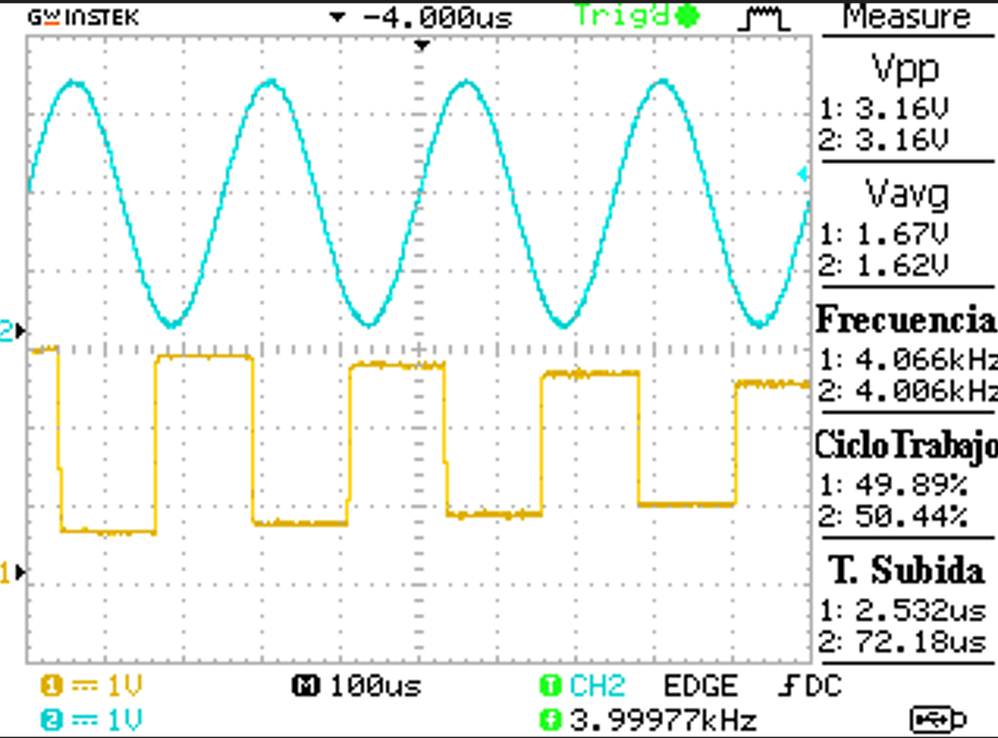
\includegraphics[width=0.7\linewidth]{8k.png}
		\caption[Medición a 8 kHz]{Medición de la señal a frecuencia de muestreo de 8 kHz}
		\label{fig:8k}
	\end{figure}
	
	
	
	
	
	
	\subsection{Análisis de los resultados obtenidos}
	
	\begin{table}[H]
		\centering
		\resizebox{\textwidth}{!}{%
			\renewcommand{\arraystretch}{1.8}
			\begin{tabular}{|c|c|c|c|c|c|}
				\hline
				\textbf{\( f_s \) [kHz]} & 
				\textbf{Muestras por ciclo (\( N \))} & 
				\textbf{\( V_{pp} \) [mV]} & 
				\textbf{\( V_{rms} \) [mV]} & 
				\textbf{THD [\%]} & 
				\textbf{SNR [dB]} \\
				\hline
				8    & 2     & 3360      & 2047.8      & 6.02      & 35.00      \\
				\hline
				16   & 4     & 3280      & 1931.5      & 8.69      & 35.59      \\
				\hline
				24   & 6     & 3280      & 1917.8      & 1.80      & 36.17      \\
				\hline
				40   & 10    & 3200      & 1943.1      & 3.58      & 36.12       \\
				\hline
				48   & 12    & 3280      & 1925.1      & 4.20      & 36.31      \\
				\hline
			\end{tabular}
		}
		\caption{Parámetros de la señal de prueba: $fs = 4 [kHz], Vpp  = 3.3[V]¨$}
		\label{tab:mediciones_senal}
	\end{table}
	
	
	\section{Conclusiones}
	La señal de prueba fue generada con un modulo AD9833, la resolución de salida es mediante un DAC de 10 bits, ademas de presentar jitter y variaciones en la amplitud pico, por lo que se podría obtener resultados mejores con un generador de funciones con mas resolución, respecto a los parámetros de las señales en todos los casos se obtiene una SNR menor a los -35 dB. Para la distorsión armónica se obtienen  valores aceptables para una velocidad de muestreo mayor a las 6 muestras por ciclo. No presenta fenómenos de aliasing ni glitches para ninguna velocidad de muestreo prevista. Ademas se midió la cantidad de ciclos por instrucciones necesarios para el procesamiento de señales arrojando el siguiente resultado:
	 
	\begin{figure}[h!]
		\centering
		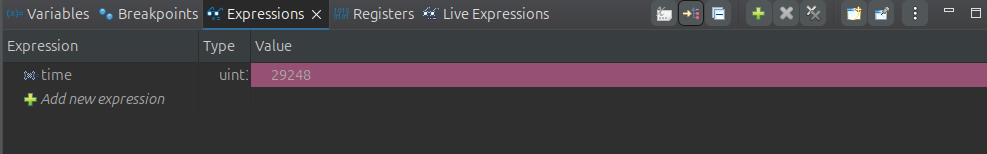
\includegraphics[width=1\linewidth]{profiling}
		\caption[Resultados modulo DWT]{Resultados modulo DWT}
		\label{fig:profiling}
	\end{figure}
	
	Si tenemos en cuenta que el microcontrolador trabaja a una velocidad de reloj de 180 MHz, podemos realizar los siguientes cálculos:
	
	\begin{equation}
		f_{CPU} = 180 [MHz]
	\end{equation}
	
	\begin{equation}
		T_{CPU} = \frac{1}{f_{CPU}} = 5.56[nS]
	\end{equation}
	
	\begin{equation}
		n_{Cycles} = 29248
	\end{equation}
	
	Por lo tanto el periodo de procesamiento es de:
	
	\begin{equation}
		T_{Processing} = T_{CPU}n°_{Cycles} = 162.59 [uS]
	\end{equation}
	
	Si tomamos el caso mas desfavorable que es cuanto la velocidad de muestreo de 48 kHz, tenemos que la ventana de tiempo del microcontrolador para realizar el procesamiento de medio buffer:
	
	\begin{equation}
		n_{Samples} = 256
	\end{equation}
	
	\begin{equation}
		T_{Sample} = \frac{1}{f_{Sample}} = 10.43 [us]
	\end{equation}
	
	\begin{equation}
		T_{threshold} = n_{Samples} T_{Sample} = 5.33[ms]
	\end{equation}
	
	Por lo tanto podemos concluir que el margen es de lo suficientemente grande como para realizar tanto el muestreo de la señal propiamente dicho así como también procesamiento adicional, el trabajo practico representa una solida base para los próximos trabajos de laboratorio que consiste en filtrado de señales, análisis espectrales, etc.
	
	\section{Bibliografía}
	
	\begin{thebibliography}{9}
		
		\bibitem{arm-cmsis-dsp}
		ARM Ltd.,
		\textit{CMSIS-DSP Software Library},
		Disponible en: \url{https://www.keil.com/pack/doc/CMSIS/DSP/html/index.html},
		[Accedido: julio 2025].
		
		\bibitem{st-datasheet}
		STMicroelectronics,
		\textit{STM32F446xC/E Datasheet - ARM Cortex-M4 32-bit MCU+FPU, 512 KB Flash, 180 MHz, ART, 3 ADCs, 2 DACs, USB OTG},
		Disponible en: \url{https://www.st.com/resource/en/datasheet/stm32f446re.pdf},
		[Accedido: julio 2025].
		
		\bibitem{st-reference-manual}
		STMicroelectronics,
		\textit{RM0390 - Reference manual STM32F446xx advanced ARM®-based 32-bit MCUs},
		Disponible en: \url{https://www.st.com/resource/en/reference_manual/dm00135183-stm32f446xx-advanced-armbased-32bit-mcus-stmicroelectronics.pdf},
		[Accedido: julio 2025].
		
		\bibitem{lyons}
		R. G. Lyons,
		\textit{Understanding Digital Signal Processing},
		3rd ed., Pearson Education, 2011.
		
		\bibitem{kubat}
		M. Kubat,
		\textit{An Introduction to Machine Learning},
		Springer, 2017. (Capítulo introductorio sobre DSP aplicado a sistemas embebidos).
		
		\bibitem{stm32cubeide}
		STMicroelectronics,
		\textit{STM32CubeIDE User Guide},
		Disponible en: \url{https://www.st.com/en/development-tools/stm32cubeide.html},
		[Accedido: julio 2025].
		
		\bibitem{stm32cubemx}
		STMicroelectronics,
		\textit{STM32CubeMX User Manual},
		Disponible en: \url{https://www.st.com/en/development-tools/stm32cubemx.html},
		[Accedido: julio 2025].
		
	\end{thebibliography}
	
	
\end{document}
